%!TEX root = practicum2.tex
\todo[inline]{Hoe verandert de fractal dimension $\rho$ als een functie van $p$? Ik het geprobeerd, zie branch fractalDimension, maar ik krijg dimensions eruit die allemaal lager zijn dan wat het hoort te zijn en het plotten gaat volledig stuk. In boxcount staat onderaan een functie de de fractal dimension berekent, op het moment gebruikt die de mean van de gradient, maar volgens Biehl zou je lineare regressie moeten gebruiken. Allebei geven ze crap resulaten.}

\textcite{falconer2004fractal} describes the fractal dimension as some number $\rho$ such that
\begin{equation}
	M_\varepsilon(\rho) \sim c\varepsilon^{-s}
\end{equation}
where $c$ and $s$ are constants and $M_\varepsilon(\rho)$ are measurements at different scales $\varepsilon$ for $\varepsilon \to 0$. \citeauthor{falconer2004fractal} then shows that the fractal dimension can be estimated ``as minus the gradient of a log-log graph plotted over a suitable range of $\varepsilon$"\cite{falconer2004fractal}. 

	% \begin{equation}
	% 	\text{dim}_{\text{box}} = \lim_{\epsilon \to 0} \frac{\log N(\epsilon)}{\log\left[ \frac{1}{\epsilon} \right]}.
	% \end{equation}
One way to get the measurements $M_\varepsilon$ is to use box-counting. When one uses this algorithm the different scales mentioned in \citeauthor{falconer2004fractal}'s definition are the sizes of the boxes.

We have used the function \t{box-count} by \textcite{boxCounting} to determine the fractal dimension of one percolation cluster. This implementation of the box-counting algorithm uses box sizes that are a power of two, consequently $\varepsilon = 1, 2, 4, \dotsc 2^q$ where $q$ is the smallest integer such that $q \leq (2N + 1)$. 

\Cref{fig:exp_fractal:cluster} shows the cluster of which we have determined the fractal dimension using box-counting. It was generated with $N = 80$, $p = 0.7$. \Cref{fig:exp_fractal:fractalDimension} presents the number of boxes as a function of the size of the boxes, \cref{fig:exp_fractal:fractalDimensionGradient} presents the minus of the gradient of \cref{fig:exp_fractal:fractalDimension}. From this graph we can infer the box-counting dimension by finding the local dimension for which the gradient is approximately stable. Using this method we find the fractal dimension to be \num{1.879}, which neatly approximates the dimension \num{1.896} mentioned by \textcite{stauffer1994introduction}. The small difference between these numbers can be explained by the relatively small size of our cluster and the fact that we present the fractal dimension of only cluster instead of the average over multiple clusters. 

\begin{figure*}
	\centering
	\begin{subfigure}[t]{0.3\textwidth}
		\centering
		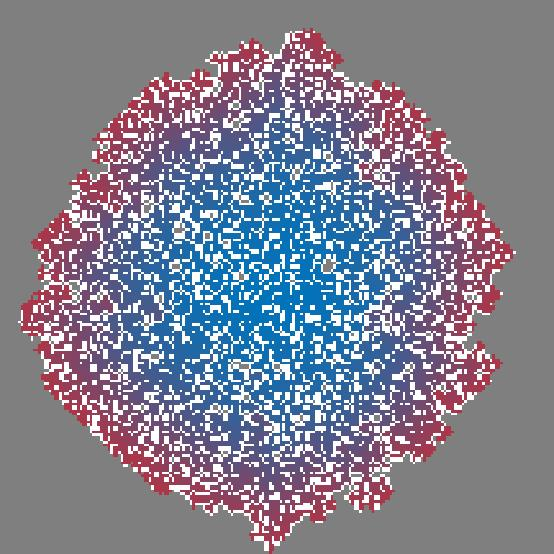
\includegraphics[width=1\textwidth]{./img/assignment_fractal_cluster}
		\caption{The cluster.}
		\label{fig:exp_fractal:cluster}
	\end{subfigure}
	\begin{subfigure}[t]{0.3\textwidth}
		\centering
		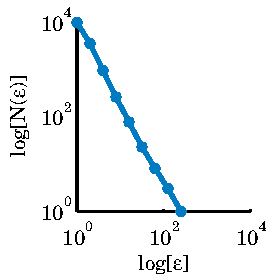
\includegraphics[width=1\textwidth]{./img/assignment_fractal_numboxesVSboxsize}
		\caption{The number of boxes as function of the box size.}
		\label{fig:exp_fractal:fractalDimension}	
	\end{subfigure}	
	\begin{subfigure}[t]{0.3\textwidth}
		\centering
		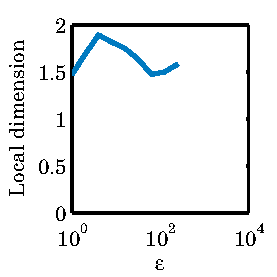
\includegraphics[width=1\textwidth]{./img/assignment_fractal_gradient}
		\caption{The minus gradient of \cref{fig:exp_fractal:fractalDimension}.}
		\label{fig:exp_fractal:fractalDimensionGradient}
	\end{subfigure}		
	\caption{\subref{fig:exp_fractal:cluster} The cluster ($N = 80, p = 0.7$) used to compute the box-counting dimension. \subref{fig:exp_fractal:fractalDimension} The number of boxes used to cover that cluster as a function of the box size. \subref{fig:exp_fractal:fractalDimensionGradient} The gradient of the function plotted in \subref{fig:exp_fractal:fractalDimension}.}
	\label{fig:exp:dimension:plaatjes}
\end{figure*}

